\chapter{Redes Neuronales Artificiales}

En este capítulo daremos una introducción a las redes neuronales artificiales veremos su uso en el aprendizaje automático para tareas de clasificación y además estudiaremos 2 tipos especiales de redes neuronales como son las \textit{redes convolucionales y recurrentes.}\\
En este seminario se dará más énfasis a las redes recurrentes y su aplicación en el procesamiento de voz para lograr la tarea de conversión voz a texto.



\section{Conceptos básicos}
A continuación describiremos algunos conceptos necesarios para el entendimiento de las redes neuronales artificiales más adelante se mostrarán nuevos de acuerdo al tipo de red.
\subsection{Neuronas}
En la biología, la neurona es conocida como la unidad fundamental del cerebro humano, el cual está compuesto por millones de neuronas interconectadas entre si(sinapsis). El trabajo de las neuronas consiste en recibir información, procesarla y enviarla a otras neuronas.\\ Este modelo fue copiado en 1943 por Warren S. McCulloch y Walter H. Pitts para poder diseñar un neurona artificial que es análoga a las neuronas del cerebro humano, esta neurona artificial tomará una cantidad n de entradas $x_{1}, x_{2}, x_{3}, .. , x_{n}$ las entradas serán multiplicadas(producto interno) por pesos $w_{1}, w_{2}, w_{3}, .. , w_{n}$ además se puede añadir una constante que llamaremos bias($b$) para producir un salida.

La entrada a la neurona será la suma total de los productos z=  $\sum_{i=1}^{n}{ w_{i}x_{i}}+b$ , el valor de z , esta se evaluará con una función f de tal forma que nuestra salida será $y=f(z)$.\\ En la ecuación 3.1 observamos la misma salida expresada en forma vectorial para nuestros vectores  $x = [x_{1}  x_{2}  x_{3}  ...  x_{n}]$ y $w = [w_{1}  w_{2}  w_{3}  ...  w_{n}]$



\begin{equation}
\label{forma vectorial}
\begin{aligned}
y&=f(x\cdot w+b)
\end{aligned}
\end{equation}
\subsection{Funciones de Activación}
La función $f$ mencionada anteriormente es una función no lineal, conocida como \textbf{función de activación.}\\ La tarea principal de la función de activación es introducir no linealidad a la salida de una neurona. Esto es importante debido a que la vida real no trabajamos solo con datos lineales y de esta forma la neurona puede aprender representaciones no lineales.\\ Entre funciones de activación tenemos algunas comúnmente usada como:
\begin{itemize}
	\item \textbf{Sigmoid}: Toma un valor real, y lo transforma en una valor en el rango de 0 a 1.\\
	$ \sigma (x) = \frac{1}{1+e^{-x}}$
	\item \textbf{tanh}: Toma por entrada un valor real y lo transfroma a un número en le rango de -1 a 1.\\
	$\tanh (x)=\frac{2}{1+e^{-x}} -1$
	\item \textbf{ReLu}: o Unidad lineal rectificada es una función que para valores menores que 0 asigna 0 y para valores mayores 
	\[   
	f(x) = 
	\begin{cases}
	\text{0} &\quad x<0\\
	\text{x} &\quad x\geq0\\

	\end{cases}
	\]
\end{itemize}
\begin{figure}[H]
	\centering
	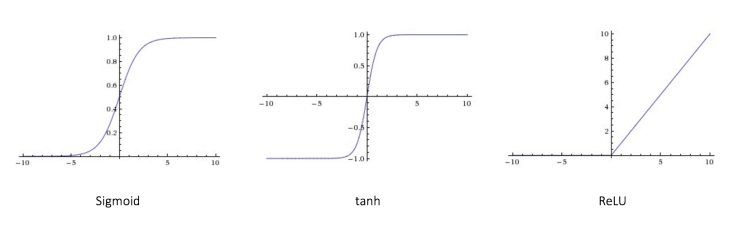
\includegraphics[width=0.9\textwidth]{Figures/factivacion.png}
	\caption{Funciones de activación \\ Fuente:  \href{https://ujjwalkarn.me/2016/08/09/quick-intro-neural-networks/}{\textit{https://ujjwalkarn.me}}}
	\label{activacion}
\end{figure} 

\subsection{Redes Neuronales Artificiales}
Las redes neuronales artificiales(ANN) toman la arquitectura del cerebro como inspiración para la construcción de sistemas inteligentes. Actualmente son la base para el desarrollo de la inteligencia artificial.\\
Una red neuronal está constituida por las uniones de neuronas.\\
En la figura 3.10 podemos ver la comparación entre una neurona biológica y un artificial etiquetadas con A y B respectivamente. Además observamos que las redes neuronales artificiales (etiqueta D) imitan el la unión biológicas de las neuronas o sinapsis(Etiqueta C).

\begin{figure}[H]
	\centering
	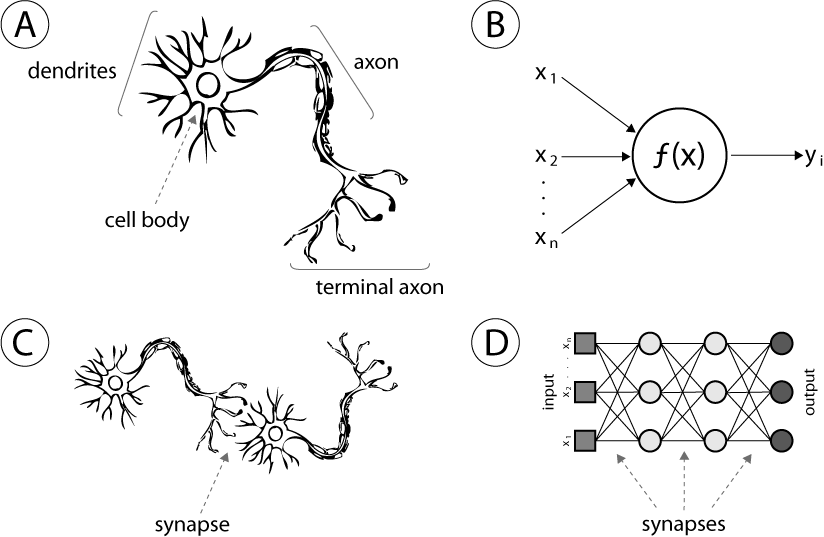
\includegraphics[width=0.8\textwidth]{Figures/ANN.png}
	\caption{Redes neuronales biológicas y artificiales \\ Fuente:  \href{https://medium.com/@ivanliljeqvist/the-essence-of-artificial-neural-networks-5de300c995d6}{\textit{https://medium.com}}}
	\label{neuronas}
\end{figure} 
\section{Redes Neuronales FeedFoward}
Estás redes fueron de las primeras y más simples. Contienen múltiples neuronas (nodos) ordenadas en capas de modo que los nodos en capas adyacentes se conectan. Cada una de estas conexiones poseen un peso asociado a dicha conexión.\\
En la figura 3.3 mostramos el esquema de Redes FeedFoward con sus distintas capas(layer).
\begin{figure}[H]
	\centering
	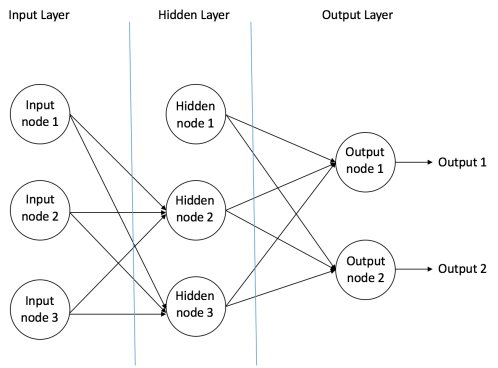
\includegraphics[width=0.5\textwidth]{Figures/esquemaff.png}
	\caption{Esquema de Redes Neuronales FeedFoward \\ Fuente:  \href{https://ujjwalkarn.me/2016/08/09/quick-intro-neural-networks/}{\textit{https://ujjwalkarn.me}}}
	\label{neuronasredes}
\end{figure} 
\begin{itemize}
	\item \textbf{Nodo de entrada(Input Node):} Proveen información a la red. En conjunto representan la capa de entrada, ningún calculo es realizado en esta capa solo se transfiere la información a la capa oculta.
	\item \textbf{Nodo Oculto(Hidden Node):} El trabajo de los nodos ocultos es calcular y transferir la información hacia a el nodo de salida. Una Red FeedFoward tiene solo una capa de entrada y una salida pero puede tener múltiples capas ocultas.
	\item \textbf{Output Node:}Su tarea principal es realizar cálculos y transferir la información fuera de la red.
\end{itemize}
En las Redes Neuronales FeedFoward, la información solo se propaga en una dirección hacia \textit{adelante} desde los nodos de entradas pasando por los nodos ocultos hacia los nodos de salida. No existen ciclos en este tipo de red.\\
Dentro de las redes neuronales FeedFoward tenemos algunos ejemplos:
\begin{itemize}
	\item \textbf{Perceptron Simple:} Es un red prealimentada simple que no posee capa oculta. Solo puede aprender de funciones lineales.
	\item \textbf{Perceptron Multicapas:} Esta red posee una o más capas ocultas. Este perceptron puede aprender de funciones no lineales.
	\item \textbf{Redes neuronales de convolución:} Este tipo de redes neuronal será explicada más adelante en el capítulo.
\end{itemize}
\subsection{Algoritmo de propagación hacia atrás}
El algoritmo de propagación hacia atrás trata de aprender de los errores, en el aprendizaje supervisado los conjuntos de entrenamiento se encuentran etiquetados. Por lo cual podemos sabemos la salida esperada. \\
El algoritmos se aplica de la siguiente forma:

\begin{enumerate}
	\item Se toma un ejemplo y se asignan pesos aleatorios a todas las conexiones de la red. Luego por medio de las conexiones y funciones de activación se calcula la salida en las capas ocultas y de salida.
	\item Se calcula el error total y se propagan estos errores hacia atrás a través de la red y se calcula la gradiente, luego se usan métodos como gradientes de descenso para ajustar los pesos y reducir el error en la capa de salida.
	\item Se repite el proceso con los otros ejemplos
\end{enumerate}
\begin{figure}[H]
	\centering
	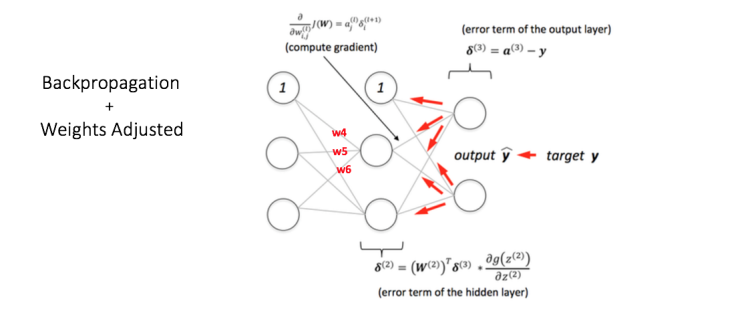
\includegraphics[width=0.9\textwidth]{Figures/backp.png}
	\caption{Propagación hacia atrás \\ Fuente:  \href{https://ujjwalkarn.me/2016/08/09/quick-intro-neural-networks/}{\textit{https://ujjwalkarn.me}}}
	\label{backpropagation}
\end{figure} 

\section{Redes Neuronales Convolucionales}
Las CNN son un tipo de Redes Neuronales FeedFoward que son especiales para procesar datos como imágenes las cuales son más difíciles de tratar en una red neuronal tradicional, como por ejemplo en el caso del perceptron multicapas.\\ El término \textit{convolucional} hace referencia a la operación lineal matemática usada. Las redes neuronales convolucionales usan esta operación para aprender de las características de mayor orden presente en los datos.
La primera CNN fue creada por Yann LeCun. Estas redes neuronales fueron inspiradas en la corteza visuales de los animales. Las células de la corteza visual, estas se activan para realizar tareas como el reconocimiento de patrones.\\  Entre sus usos más comunes tenemos el reconocimiento de imágenes y lenguaje natural.\\
\subsection{Estructura de una imagen}
Debido a que las redes neuronales convolucionales son usadas comúnmente con imágenes, es importante conocer cual es la estructura de una imagen y cómo es que la computadora comprende y utiliza esta información.\\
Las imágenes están constituidas por una sucesión de píxeles, podemos entender el pixel como la menor unidad homogénea en color de una imagen digital. Teniendo este concepto, podemos dividir la información de una imagen de la siguiente forma:
\begin{itemize}
	\item \textbf{Width}: El ancho de la imagen medido en pixeles
	\item \textbf{Height}: El alto de la imagen medida en pixeles.
	\item \textbf{Canales RGB}: Estos canales contiene la información de los colores y profundidad de una imagen. Este canal guarda la información en tres canales Red, Green y Blue.
\end{itemize}

\begin{figure}[H]
	\centering
	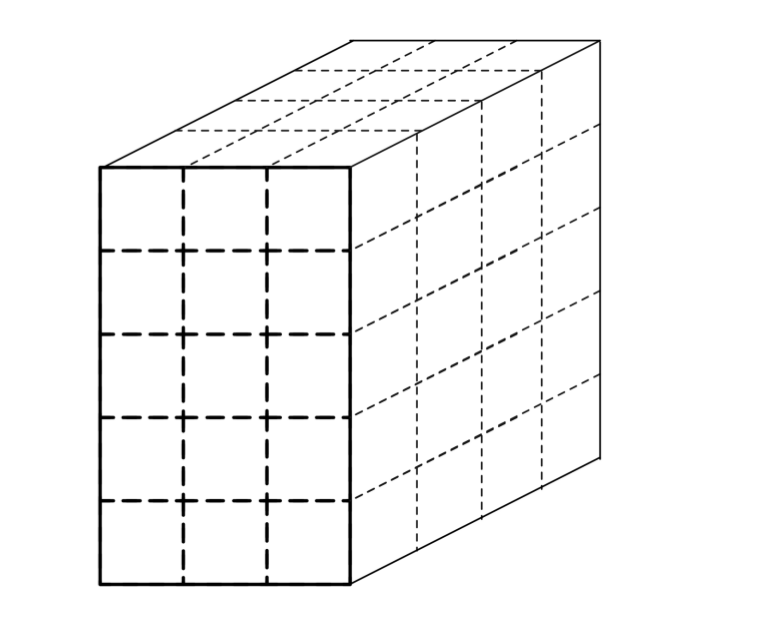
\includegraphics[width=0.7\textwidth]{Figures/image.png}
	\caption{Estructura de la imagen de entrada \\ Fuente:  \href{https://www.safaribooksonline.com/library/view/deep-learning/9781491924570/ch04.html}{\textit{Deep Learning by Adam Gibson, Josh Patterson}}}
	\label{image}
\end{figure} 

Teniendo en cuenta esta forma de dividir la información de una imagen podemos resaltar la ventaja de usar Redes convolucionales en lugar de usar una red neuronal multicapas.\\ Las redes multicapas toman un vector de una dimensión como entrada, si quisiéramos entrenar un perceptron multicapas con imágenes de 32x32 píxeles y con 3 canales RGB necesitaríamos crear 3072 pesos ($w_{i}$) para una sola neurona en la capa oculta. Esta generación excesiva de peso hace que la tarea resulte complicada usando redes multicapas.\\ De esta forma surge la idea de recurrir a un tiempo tipo de redes neuronales que faciliten la tarea sin consumir muchos recursos.
\subsection{Capas de una CNN}
Las redes neuronales convoluciones pueden ser dividas en distintas capas, cada una de ellas con una tarea específica para el tratamiento de la información. En esta sección describiremos cada una de estas capas.
\subsubsection{Input layer}
Esta capa es la encargada de cargar y almacenar la información de las imágenes para luego procesarlas en la red. Esta información contiene detalles de ancho, alto en píxeles y el número de canales de imagen. Las entradas de esta capa corresponden a la imagen vista en la figura 3.5.

\subsubsection{Convolutional layers}
Es una de las capas más importante en el diseño de las CNNs, esta capa es la encargada de transformar la entrada(imagen o convolución anterior) usando las conexiones de las neuronas en capas anteriores. 

Para entender más a fondo esta capa debemos definir la operación de \textit{convolución}.\\  La \textit{convolución} es una operación matemática que describe una regla de como fusionar 2 conjuntos de información.\textquotedblleft  Esta operación tiene importancia en campos como la matemática y la física debido que permite definir un puente entre el domino del espacio/tiempo y el dominio de la frecuencias a través del uso de la transformada de fourier.
La convolución toma una entrada, aplica un kernel de convolución y nos da un mapa de características como salida \textquotedblright \cite{book1} .\\
Las convoluciones son usadas principalmente como un detectores de características cuyas entradas son la capa de entrada u otra convolución.
En la figura 3.6 observamos la operación de convolución que por medio del uso de un kernel o filtro de convolución extrae características de la imagen, por ejemplo detalles como bordes de una imagen.\\ Haciendo analogía con los pesos en las redes neuronales convencionales, las redes convolucionales poseen el \textit{ filtro o kernel }, esto resulta beneficioso, ya que no se tendrá definir un peso para cada neurona.\\ El kernel de la figura 3.6 será desplazado a lo largo de las dimensiones espaciales. Durante el desplazamiento, el kernel se multiplicará por los datos de entrada dentro de su limite, produciendo una sola salida al mapa de características.
\begin{figure}[H]
	\centering
	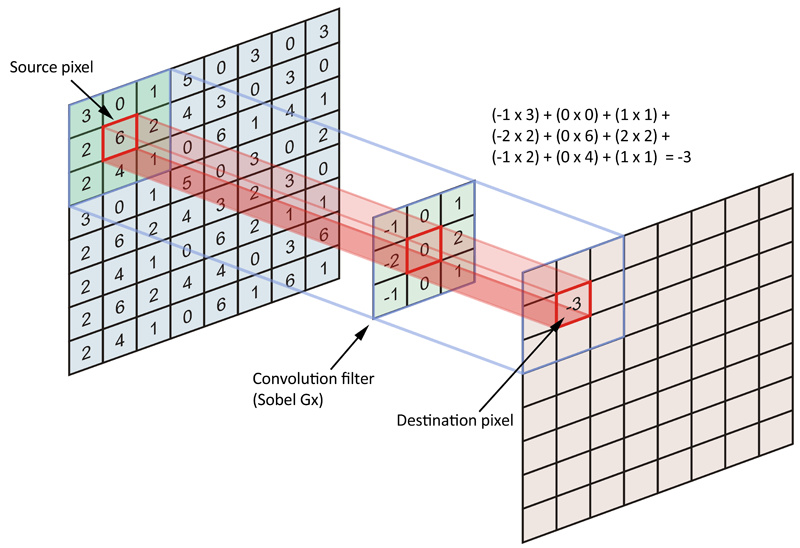
\includegraphics[width=0.8\textwidth]{Figures/convolucion.jpeg}
	\caption{Operacion de convolución \\ Fuente:  \href{http://openresearch.ai/t/network-in-network/39}{\textit{www.openresearch.ai}}}
	\label{convolucion}
\end{figure} 

Las capas convolucionales aplican transformaciones o funciones de activación al conjunto de entrada, luego el mapa de activación generado se apilará a lo largo de dimensión de profundidad para construir el volumen de salida.

\textbf{Componentes de la capa de convolución}.\\	\\
Las capas convolucionales poseen parámetros e hiperparámetros. La gradiente de descenso tiene la funcion de entrenar a estos parámetros de modo que las clases sean consistentes con las etiquetas en el conjunto de entrenamiento. Entre estos parámetros tenemos:
\textbf{Filtros}

Los filtros son una función que posee ancho(width) y alto (height) más pequeños que la entrada. Los filtros son aplicados a través de  del ancho y alto de la entrada, pero también pueden ser aplicados a lo largo de la profundidad.

\vspace{5cm}
\textbf{Hiperparámetros de una capa de convolución}.\\
A continuación veremos algunos hiperparámetros que determinan la disposición espacial y tamaño del volumen de salida de una capa convolucional.
\begin{itemize}
	\item \textbf{Filter size:} Cada filtro es pequeño con respecto al ancho(width) y alto(height) del la capa anterior. Por ejemplo podemos tener un filtro de tamaño $[5x5x3]$, lo representa 5 de ancho x 5 de alto x 3 de los canales RGB.
	\item \textbf{Output depth:} Este hiperparámetro controla el número de neuronas en la capa convolucional que están conectadas al mismo del volumen de entrada. Este parámetro puede ser elegido manualmente.
	\item \textbf{Stride:} Se encarga de configurar el tamaño de desplazamiento de la ventana de filtro. Cada filtro aplicado a la columna de entrada asignará más profundidad en el volumen de salida. Un stride grande creará un volumen de salida más grande y uno valor pequeño obtendrá un volumen menor.
	\item \textbf{Zero-padding:} Con este parámetro se puede controlar el volumen de salida. Es usado para mantener el tamaño espacial de entrada en la salida. 
\end{itemize}

\subsubsection{Pooling layers}
Este tipo de capas se encuentran entre las capas convolucionales. Se encarga de reducir el tamaño espacial(ancho,alto) de los datos de representación. Esta capa reduce la representación de los datos progresivamente a través de la red y ayuda a controlar el \textit{overfitting}.\\
Esta capa utiliza la operación \textit{max()} para cambiar el tamaño de los datos de entrada espacialmente, a esta operación se le conoce como max pooling. Esta funciona de siguiente forma toma un filtro de $n x n$, y la operación $max$ toma el mayor de los números en el área de filtro.\\ \\ Por ejemplo en caso tener una imagen de entrada $32 \times 32$ píxeles y se aplica un filtro de $2\times2$, como resultado obtendremos una salida de $16\times16$ píxeles. Esto reduce cada segmento de profundidad en el volumen de entrada por un factor de 2.

\subsubsection{Fully Connected Layers}

Esta capa se calcula el puntaje de las clases que usaremos como salida de red, esta será la encargada de reconocer a que clase pertenece una imagen de prueba de acuerdo a su puntaje o probabilidad. Las dimensiones del volumen de la salida son [1x1xN], donde el valor de N corresponde al número de clases de salida que se están evaluando. En el caso del MNIST (dataset para reconocimiento de dígitos), el valor de N es igual a 10, número que corresponde a los 10 dígitos distintos que posee el dataset($0, ... ,9$).\\
Esta capa tiene conexión entre todas sus neuronas y las de la capa anterior. Esta capa realiza las transformaciones del volumen de datos de entrada. Estas son funciones de activación en el volumen de entrada y los parámetros (pesos y bias de las neuronas).
\vspace{2cm}
\subsection{Arquitecturas conocidas}
Actualmente existen algunas arquitecturas de CNN ya diseñadas que son aplicadas para el trabajo de reconocimiento de imágenes.\\ El proyecto ImageNet, posee una gran base de datos de imágenes. Este proyecto realizá una competición llamada \textit{ImageNet Large Scale Visual Recognition Challenge (ILSVRC) } donde compiten distintos programas de software para detectar y clasificar objetos.\\ A continuación mostraremos algunas de las arquitecturas más importante de esta competencia:

\begin{itemize}
	\item \textbf{LeNet-5 (1998)} \textquotedblleft Arquitectura propuesta por LeCun, consiste 2 capas de convolución, activación  y capas pooling seguidas por a fully conected layer\textquotedblright \cite{WEBSITE:9}
	\vspace{1cm}
	\item \textbf{AlexNet (2012)} Fue propuesta por Alex Krizhevsky, esta arquitectura posee 5 capas de convolución seguida por 3 fully connected layers.
	\vspace{1cm}
	\item \textbf{VGGNet (2014)} Fue desarrollada para Sigmoyan y Zisserman para la competición ILSVRC. \textquotedblleft VGG consta de 16 capas convolucionales y es muy atractivo debido a su arquitectura uniforme. Consta de convoluciones de 3x3 y utiliza múltiples filtros \textquotedblright \cite{WEBSITE:10}	
\end{itemize}

\section{Redes Recurrentes}
Las redes neuronales recurrentes aparecieron en los años 1980s, actualmente se han desarrollado más estudios debido a la mejora de hardware. Son utilizadas principalmente para tratar con una información de secuencia, por ejemplo series de tiempo, audio, sentencia de oraciones, etc.\\ La principal diferencia de la redes con las redes neuronales feed-foward es que en las neuronas de las redes recurrentes las salidas regresan a la entrada de esta manera mantiene información de un estado anterior. Esto permite que nuestro modelo sea cambiante cada vez que este se alimente con una secuencia nueva.%%\subsubsection*{Características}

Dentro de una capa recurrente se tiene los siguientes tipos de conexiones :
\begin{itemize}
	\item  \textbf{Entrantes:} Son aquellas que emanan de la capa previa.
	\item  \textbf{Salientes:} Estas conexiones son dirigidas a todas las neuronas de las capas consecuentes.
	\item  \textbf{Recurrentes:} se encargan de propagar la información entre las neuronas de las misma capa.
\end{itemize}


\begin{figure}[H]
	\centering
	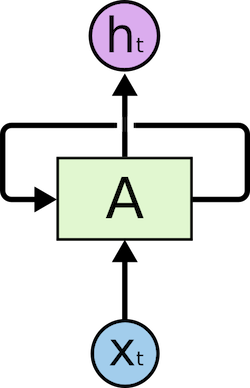
\includegraphics[width=0.3\textwidth]{Figures/rnn.png}
	\caption{Neurona Recurrente \\ Fuente:  \href{https://cdn-images-1.medium.com/max/960/1*XB5c4rTCSeFQrK0aFC5IVw.png}{\textit{https://medium.com}}}
	\label{}
\end{figure}

Es posible representar a la redes recurrentes como si fueran redes feed-fowards esto lo realizamos \textit{desenrrollando} la neurona como vemos en la figura 3.8 el $x_{t}$ representa un estado final de esta forma podemos representar la red como un conjunto de estados a través de un lapso de tiempo. En esta forma las técnicas de backpropagation pueden ser usadas en la redes recurrentes.

\begin{figure}[H]
	\centering
	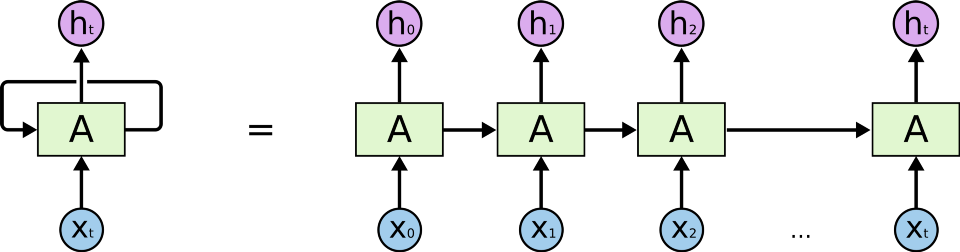
\includegraphics[width=0.9\textwidth]{Figures/rnn2.png}
	\caption{Versión desenrollada \\ Fuente:  \href{https://towardsdatascience.com/introduction-to-recurrent-neural-network-27202c3945f3}{\textit{https://towardsdatascience.com}}}
	\label{}
\end{figure}
\newpage
\subsection{Propagación hacia atrás través del tiempo(BPTT)}

Las redes neuronales feedfoward, la propagación hacia atrás se encarga de transmitir el error de la salida hacia a las capas ocultas asignados a los pesos(w) responsabilidad del error general mediante el uso de la derivada parcial $\frac{ { \partial } E } { \partial w }$. En estas redes es común usar la propagación hacia atrás debido a que el par entrada salida posee un tamaño fijo situación que no ocurre con las secuencia de datos.\\
 Las redes neuronales recurrentes utilizan una extensión de la propagación hacia atrás llamada \textit{Propagación hacia atrás a través del tiempo}, o BPTT  por sus siglas en inglés, la cual se aplica para secuencia de datos.
Este algoritmo consta de los siguiente pasos:
\begin{itemize}
	\item Dado unos lapsos de tiempo entre la entrada y la salida de la red.
	\item Se desenrolla la red(Ver Figura 3.8) , calcula y acumulada los errores de cada lapso de tiempo.
	\item Enrolla la red y actualiza los pesos para reducir el error.
	
\end{itemize}

\textquotedblleft Si la secuencia de datos consta de 1000 lapsos de tiempo, este será el número de derivadas requeridas para una simple actualización \textquotedblright \cite{WEBSITE:20}

\begin{figure}[H]
	\centering
	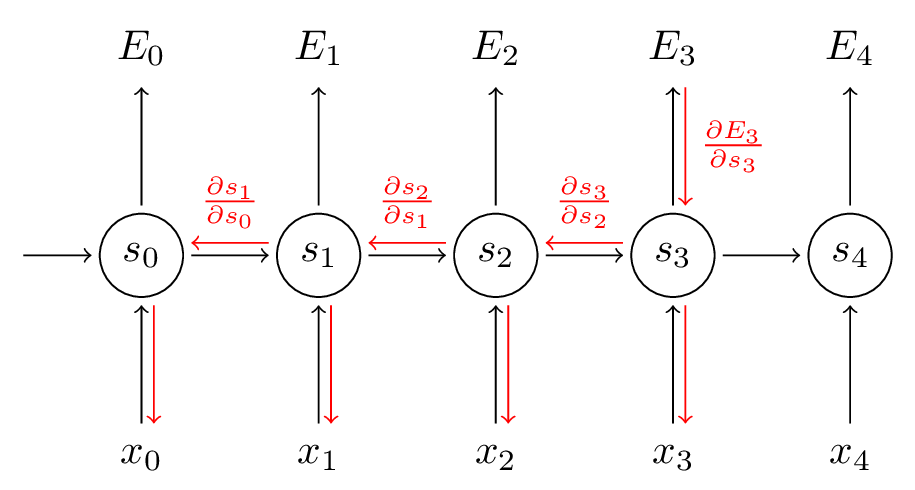
\includegraphics[width=0.8\textwidth]{Figures/BPTT1.png}
	\caption{BPTT \\ Fuente:  \href{http://www.wildml.com/2015/10/recurrent-neural-networks-tutorial-part-3-backpropagation-through-time-and-vanishing-gradients/}{\textit{http://www.wildml.com}}}
	\label{}
\end{figure}

En este esquema de básico de redes neuronales recurrentes utilizamos la función de activación softmax para calcular los valores de la celda y utilizamos pesos($U,W,V$) de esta forma tenemos que:
\begin{equation}
	\label{ST}
	\begin{aligned}
	s_{t}&=\tanh(Ux_{t}+Ws_{t-1})\\
	\hat{y}_{t}&=softmax(Vs_{t})
	\end{aligned}
\end{equation}
Donde $s_{t}$ son los valores de la celda y $\hat{y}_{t}$ es la predicción. A continuación calcularemos el error de nuestra red utilizando el valor de la predicción $\hat{y}_{t}$ y el valor real $y_{t}$.
\begin{equation}
	\label{STs}
	\begin{aligned}
		E_{t}(y_{t},\hat{y_{t}})&=y_{t}logy_{t}\\
		E_{t}(y,\hat{y})&=\sum_{t}{E_{t}(y_{t},\hat{y_{t}}}\\
	\end{aligned}
\end{equation}
Nuestro objetivo será ajustar los pesos ($U,W,V$) por lo cual usaremos la gradiente de descenso con respecto a los pesos los cuales serán calculados en la ecuación 3.4.

\begin{equation}
\label{Ts}
\begin{aligned}
	\frac{\partial E}{\partial W}&=\sum_{t}{\frac{\partial E_{t}}{\partial W}}
\end{aligned}
\end{equation}
Para calcula esta gradiente haremos uso de la regla de la cadena para simplificar los cálculos usaremos un ejemplo el $E_{t}$ para $t=2$.


\begin{equation}
\label{Tsfs}
	\begin{aligned}
	\frac{\partial E_{2}}{\partial V}&=\frac{\partial E_{2}}{\partial \hat{y_{2}}} \frac{\partial \hat{y_{2}}}{\partial V}\\
	\frac{\partial E_{2}}{\partial V}&=\frac{\partial E_{2}}{\partial \hat{y_{2}}} \frac{\partial \hat{y_{2}}}{\partial z_{2}} \frac{\partial \hat{z_{2}}}{\partial V}\\
	\frac{\partial E_{2}}{\partial V}&=(\hat{y_{2}}-y_{2})\otimes s_{3}
	\end{aligned}
\end{equation}
Donde $s_{2}=Vs_{3}$ ahora calcularemos para W como $s_{2}=tanh(Ux_{t}+ Ws_{1})$
Al derivar obtenemos la ecuación 3.6 luego se sumarán las contribuciones en cada lapso de tiempo.
\begin{equation}
\label{TsSfs}
	\begin{aligned}
		\frac{\partial E_{2}}{\partial W}&=\frac{\partial E_{2}}{\partial \hat{y_{2}}} \frac{\partial \hat{y_{2}}}{\partial s_{2}} \frac{\partial \hat{s_{2}}}{\partial s_{k}} \frac{\partial s_{k}}{\partial W}
	\end{aligned}
\end{equation}

\subsection{Desaparición de la gradiente}
Las redes recurrentes ofrecen una gran ventaja al manejar \textit{secuencias de datos} pero el trabajar con este tipo de datos también pueden repercutir en un problema conocido como la desaparición de la gradiente, o \textit{Vanishing Gradient}, el cual es una de la principales dificultades en las redes recurrentes.\\
 La gradiente de descenso nos permite actualizar los valores de nuestros pesos para que nuestra red continué aprendiendo, pero si esta gradiente desaparece, debido a que toma un valor pequeño, nuestra red deja de aprender en términos sencillos en esto consiste el problema de \textit{desaparición de gradiente}.

Dado que en la propagación hacia atrás se calcula la gradiente usando la regla de la cadena podemos suponer que usamos la función sigmoid de la figura 3.9 notamos que su derivada para valores positivos y negativos grandes toma el valor de 0 lo que producirá que la gradiente desaparezca y nuestra red deje de aprender al no poder actualizar.

Entre la soluciones para este problema se encuentran usar otras funciones de activación como Relu o Elu, también se pueden usar métodos de normalización para los batchs.
\begin{figure}[H]
	\centering
	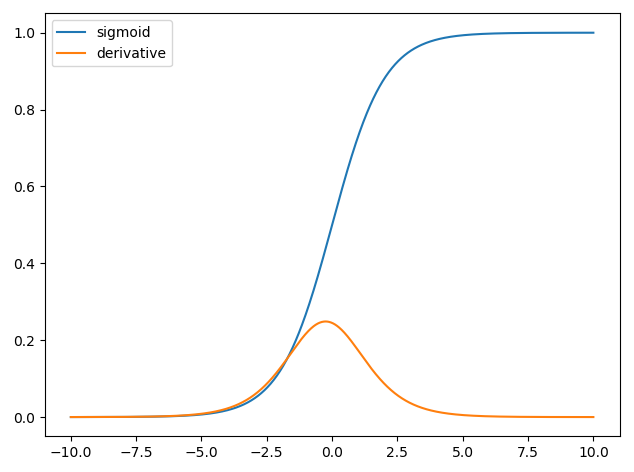
\includegraphics[width=0.5\textwidth]{Figures/sigmoid.png}
	\caption{Función sigmoid y su derivada \\ Fuente:  \href{https://cdn-images-1.medium.com/max/960/1*XB5c4rTCSeFQrK0aFC5IVw.png}{\textit{https://medium.com}}}
	\label{}
\end{figure}

\subsection{Long Short Term Memory (LSTM)}

LSTM es un tipo de red neuronal recurrente que fue propuesto por Sepp Hochreiter y Jurgen Schmidhuber.\cite{LSTM} para aprovechar las ventajas de las redes recurrentes y combatir el problema de la desaparición de gradiente.\\ En la redes recurrentes se trasmite la información pero ha medida que transcurre el tiempo están son olvidadas, a esto se le llamó el \textit{problema de las dependencias a largo plazo}. Las LSTM buscan solucionar este problema, por lo cual estas se encargan de transmitir la información y \textit{recordarla} mientras los lapsos de tiempo pasan imitando la \textit{capacidad de la memoria humana para recordar.}


\begin{figure}[H]
	\centering
	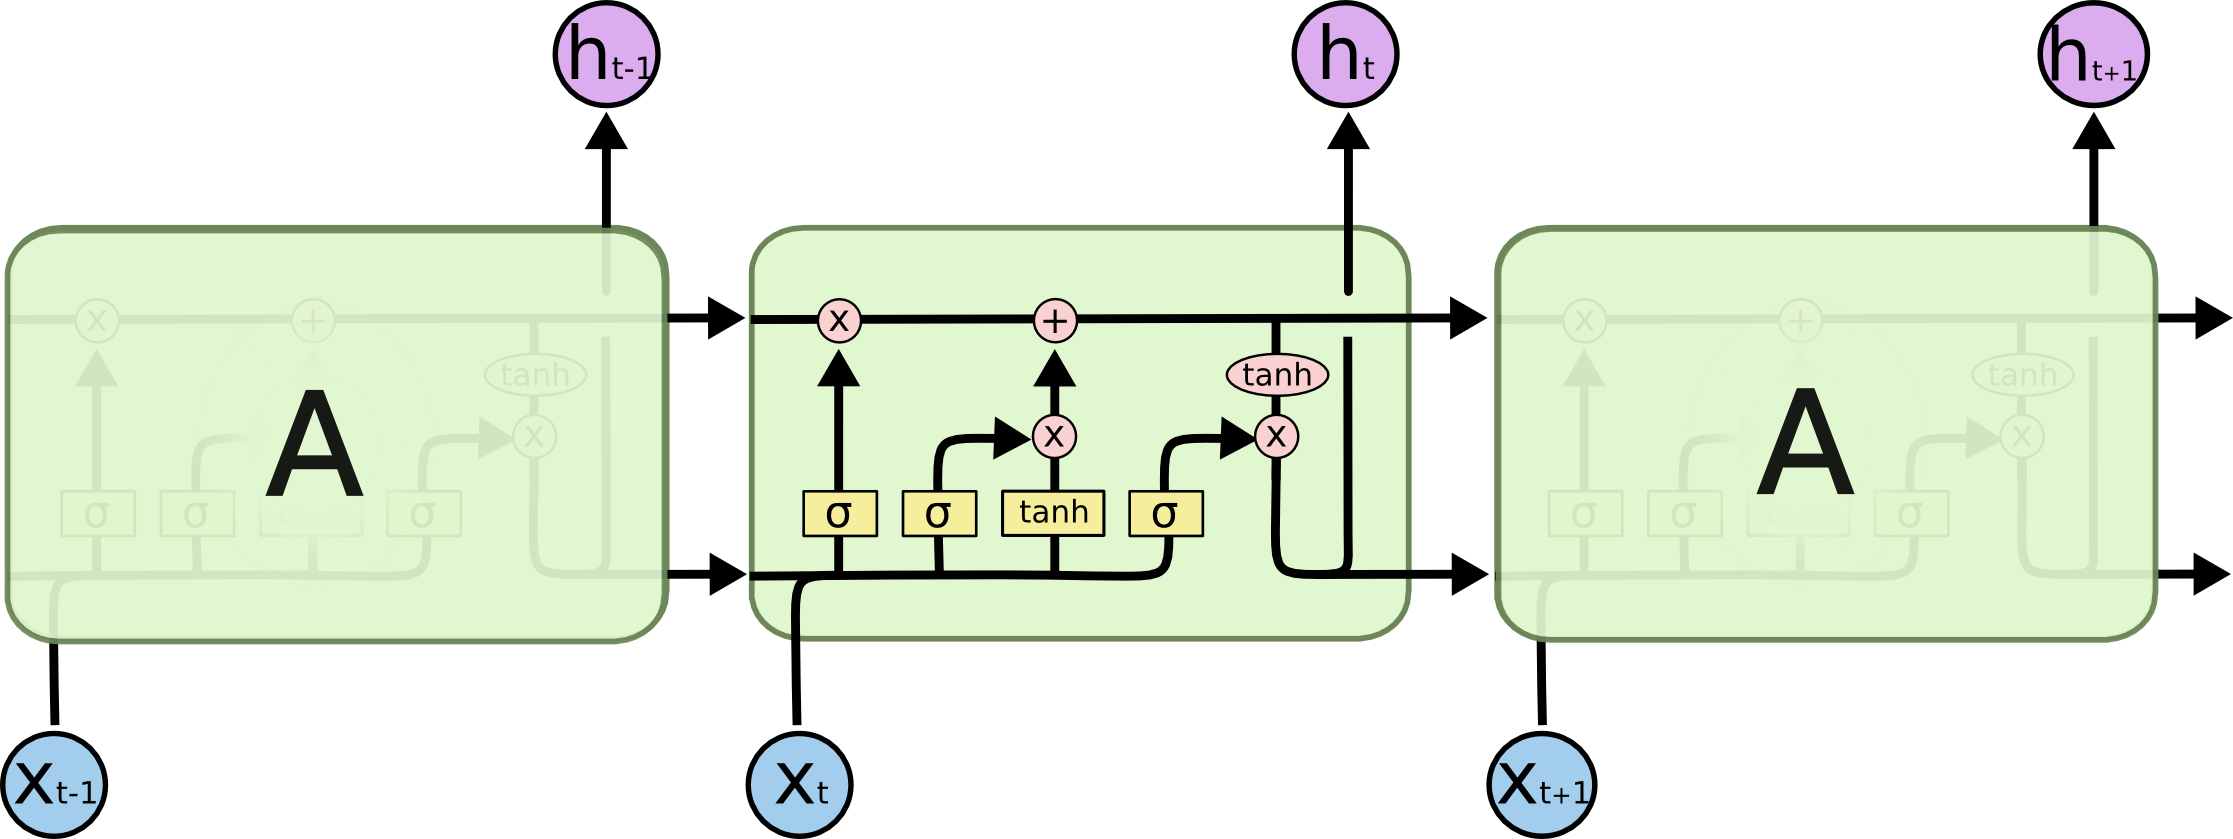
\includegraphics[width=0.8\textwidth]{Figures/LSTM-chain.png}
	\caption{Estructura en cadena \\ Fuente:  \href{http://colah.github.io/posts/2015-08-Understanding-LSTMs/}{\textit{http://colah.github.io}}}
	\label{}
\end{figure}

En la siguiente figura observamos el esquema de una unidad, o neurona, de LSTM y estudiaremos su comportamiento.
\begin{figure}[H]
	\centering
	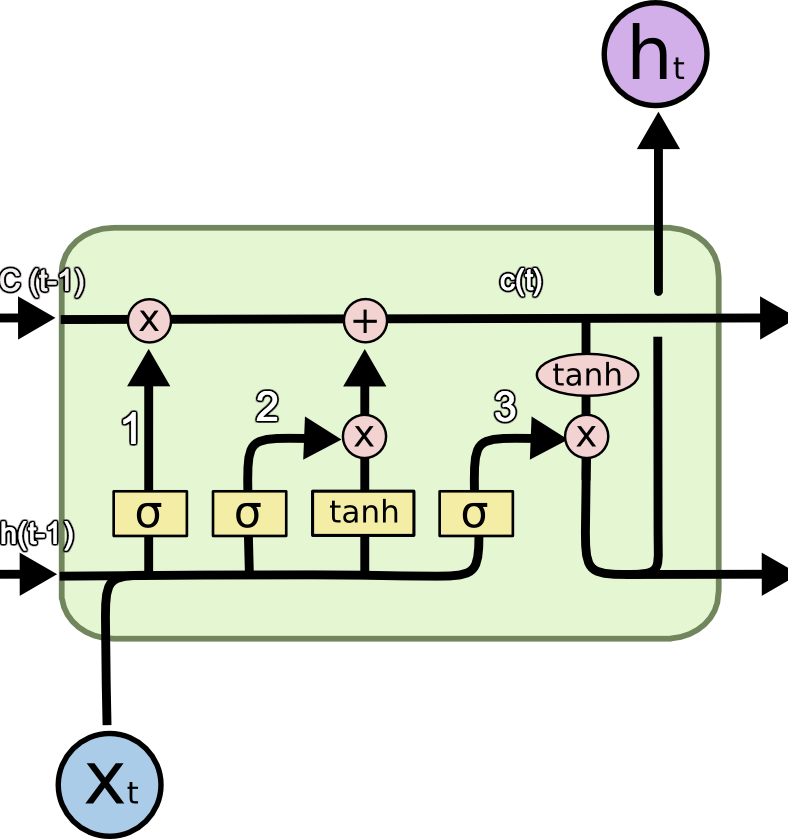
\includegraphics[width=0.4\textwidth]{Figures/LSTM.png}
	\caption{Unidad de LSTM \\ Fuente:  \href{https://towardsdatascience.com/understanding-lstm-and-its-quick-implementation-in-keras-for-sentiment-analysis-af410fd85b47g}{\textit{https://towardsdatascience.com}}}
	\label{}
\end{figure}

\begin{itemize}
	\item $X_{t}$: entrada actual
	\item $\sigma$: capa sigmoid
	\item $tanh$: capa tanh
	\item $h_{t-1}$: salidas de la última unidad.
	\item $C_{t-1}$: memoria de la última unidad.
	\item $h_{t}$: salida actual.
	\item $C_{t}$: memoria actualizada
	
\end{itemize}


Principalmente la idea de LSTM gira entorno a las celdas de estado  $c_{t}$, esta será la encargada de añadir nueva información o removerla si ya no es necesaria.

\begin{figure}[H]
	\centering
	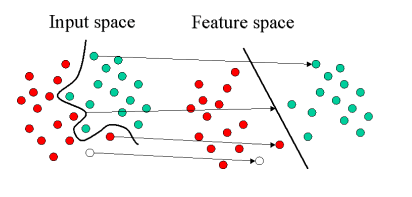
\includegraphics[width=1\textwidth]{Figures/kernel.png}
	\caption{celda de estado \\ Fuente:  \href{http://colah.github.io/posts/2015-08-Understanding-LSTMs/}{\textit{http://colah.github.io}}}
	\label{}
\end{figure}

El valor de la celda de estado($C_{t}$) y la salida($h_{t}$) :
\begin{enumerate}
	\item  Nuestro LSTM decidirá que información será desechada de nuestra célula de estado. Esta decisión utilizará una capa sigmoidal llamada \textit{forget gate layer} la cual genera un número entre 0 y 1, lo cual definirá la cantidad de información que mantendrá.
	\begin{figure}[H]
		\centering
		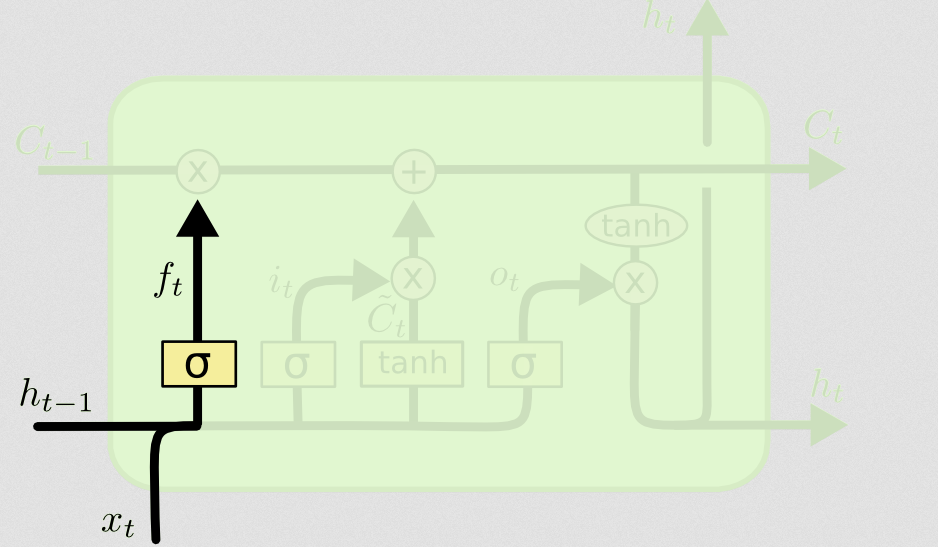
\includegraphics[width=0.75\textwidth]{Figures/forgetay.png}
		\caption{capa sigmoidal \\ Fuente:  \href{http://colah.github.io/posts/2015-08-Understanding-LSTMs/}{\textit{http://colah.github.io}}}
		\label{}
	\end{figure}
			\begin{equation}
				\label{forget layer}
				\begin{aligned}
				f_{t}&=\sigma(W_{t}\cdot[h_{t-1},x_{t}]+b_{f})
				\end{aligned}
			\end{equation}
	\item Una vez que se ha olvidado es importante es aceptar nueva información y almacenarla. Esto será realizado en los siguientes pasos.
	\begin{enumerate}
		\item Una capa sigmoid llamada \textit{input gate layer} decide que valores serán actualizados($i_{t}$).

	

		\item Una capa tanh crea un vector de valores posibles, o valores candidatos, $\hat{C}_{t}$ .
		\begin{figure}[H]
			\centering
			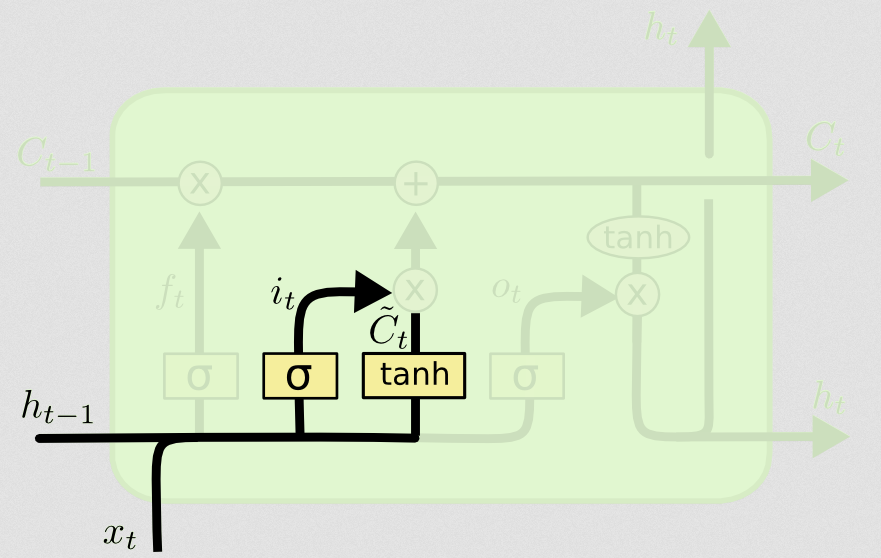
\includegraphics[width=0.75\textwidth]{Figures/forgetay2.png}
			\caption{capa tanh \\ Fuente:  \href{http://colah.github.io/posts/2015-08-Understanding-LSTMs/}{\textit{http://colah.github.io}}}
			\label{}
		\end{figure}
		\begin{equation}
			\label{forget layer}
			\begin{aligned}
			i_{t}&=\sigma(W_{i}\cdot[h_{t-1},x_{t}]+b_{i})\\
			\hat{C}_{t}&=\sigma(W_{C}\cdot[h_{t-1},x_{t}]+b_{C})
			\end{aligned}
			\end{equation}
		\item Finalmente se combinan ambos para actualizar la celda de estado.
		\begin{figure}[H]
			\centering
			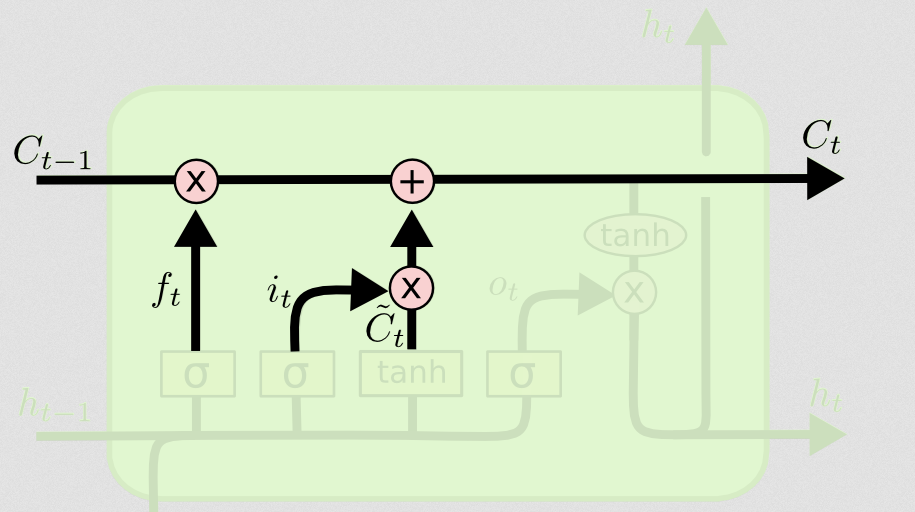
\includegraphics[width=0.6\textwidth]{Figures/LSTM8.png}
			\caption{Actualización del $C_{t}$ \\ Fuente:  \href{http://colah.github.io/posts/2015-08-Understanding-LSTMs/}{\textit{http://colah.github.io}}}
			\label{}
		\end{figure}
		\begin{equation}
			\label{ctlayer}
			\begin{aligned}
				C_{t}&=f_{t}\ast C_{t-1} + i_{t}\ast \hat{C}_{t}
		    \end{aligned}
		\end{equation}
	\end{enumerate}
\item Finalmente para obtener la salida de este módulo $C_{t}$
		\begin{figure}[H]
	\centering
	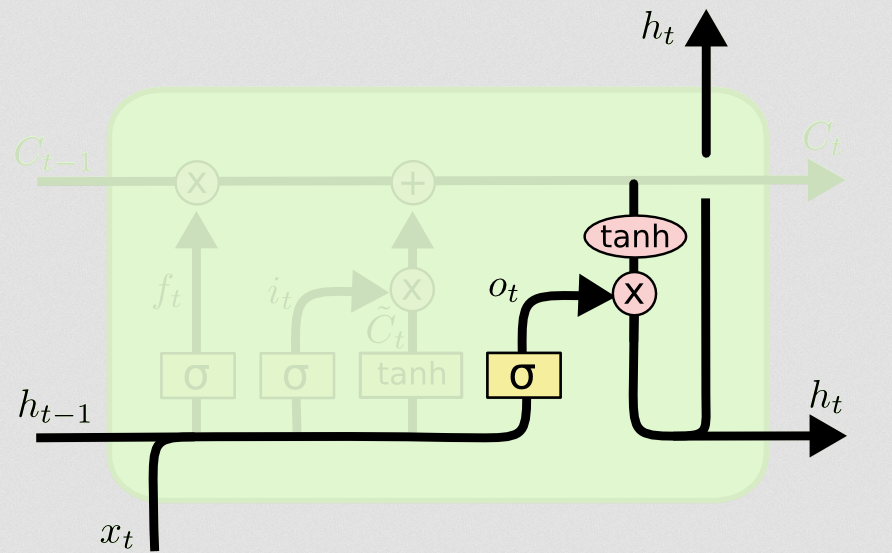
\includegraphics[width=0.75\textwidth]{Figures/LSTM9.png}
	\caption{Calculo del $h_{t}$ \\ Fuente:  \href{http://colah.github.io/posts/2015-08-Understanding-LSTMs/}{\textit{http://colah.github.io}}}
	\label{}
\end{figure}
		\begin{equation}
			\label{ht}
			\begin{aligned}
				o_{t}&=\sigma(W_{o}[h_{t-1},x_{t}]+b_{o})\\
				h_{t}&=o_{t}\ast \tanh(C_{t})
			\end{aligned}
		\end{equation}
\end{enumerate}

\newpage
Una variante de las redes recurrentes son las redes recurrentes bidireccionales, la cual consiste en aprender de una secuencia de datos en 2 direcciones siguiendo lapsos de tiempo de la secuencia hacia adelante y atrás. Al capturar la información de la secuencia invertida nos permite mejorar nuestra predicción.	\textquotedblleft Para superar las limitaciones de una RNN regular proponemos un modelo bidireccional de redes recurrentes(BRNN) la cual puede ser entrenada con la información de entrada en el pasado y en el futuro de un marco especifico de tiempo \textquotedblright \cite{BRNN}


%%%
%%\begin{figure}[H]
%%\centering
%%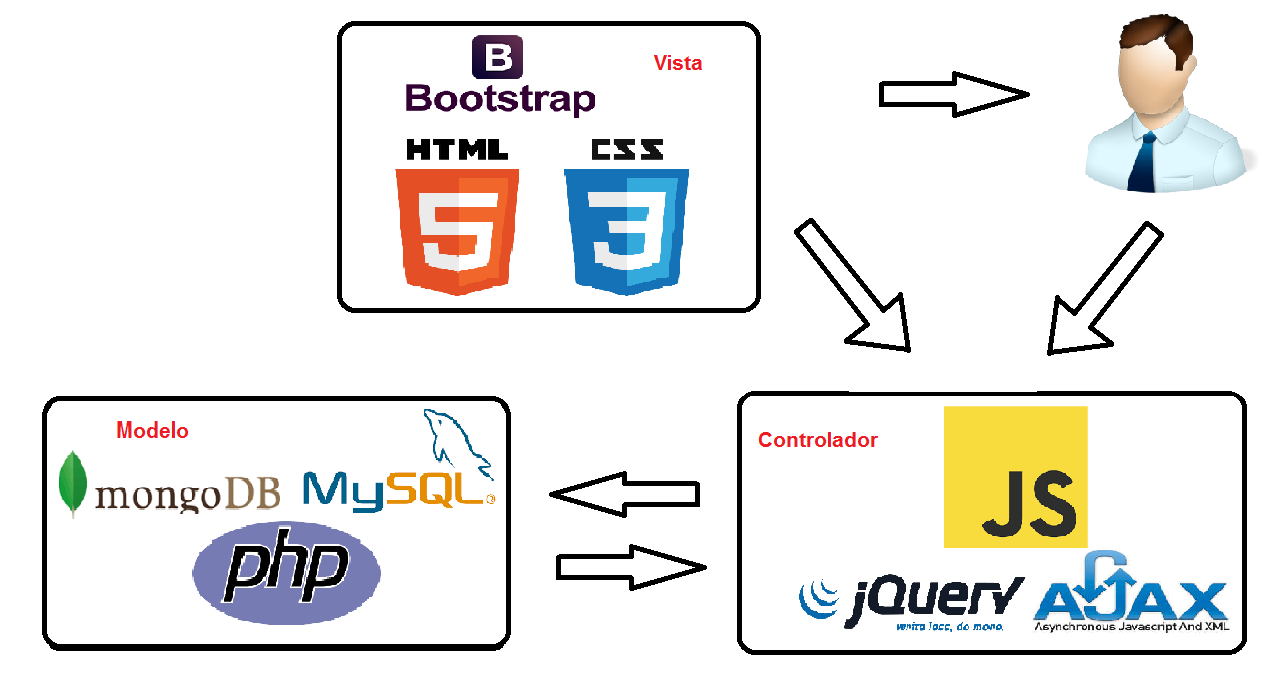
\includegraphics[width=0.9\textwidth]{Figures/mvc.png}
%%\caption{Modelo-Vista-Conrolador}
%%\label{MVC}
%%\end{figure}



